The efforts of the first reporting period have have been mainly focused on creating the adequate tools to manage the information resulting of the project evolution and to handle the discussions and on learning about the existing BuB initiatives and make the initial contact with some of them.

\subsection{Tools for BuBforEurope}
\label{tools}

The tools set up are websites and mailing lists. While generally mailing lists are meant for discussions and direct communication, websites are meant for longer term and more elaborated contents. All the tools are hosted at Community Networks (CNs) servers and managed by CNs members. All the contents are publicly available.

\subsubsection{BuB mailing list}

\url{https://llistes.guifi.net/sympa/info/bub}

Hosted at guifi.net's mailing list manager\footnote{Sympa \url{http://www.sympa.org/}.}, this public list was the first public mean of communication set up. Started on May 2012, as of October 2013 it has over 500 mails in total and 59 subscribers, half of them without any kind of affiliation with the Commons for Europe partners. It has become the place the facto to discuss not only about BuBforEurope but also about more general BuB issues. For instance, all project pilot's management (announcements, discussions, etc.) is done via this mailing list.


\subsubsection{BuBforEurope website}

\url{http://bubforeurope.net/}

This website hosted at a guifi.net's data centre\footnote{Telvent's PoP, Barcelona. See \emph{D5.4.2 Report on Pilots on Fiber Deployment -- a}.}. Operational since January 2013 is aimed gathering all the information of BuBforEurope. It is a Drupal\footnote{\url{https://drupal.org/}} based website with the wiki, news, forums and forms modules enabled. Firgure~\ref{fig:bub_web} shows the website main page.

\begin{figure}[H]
  \centering
  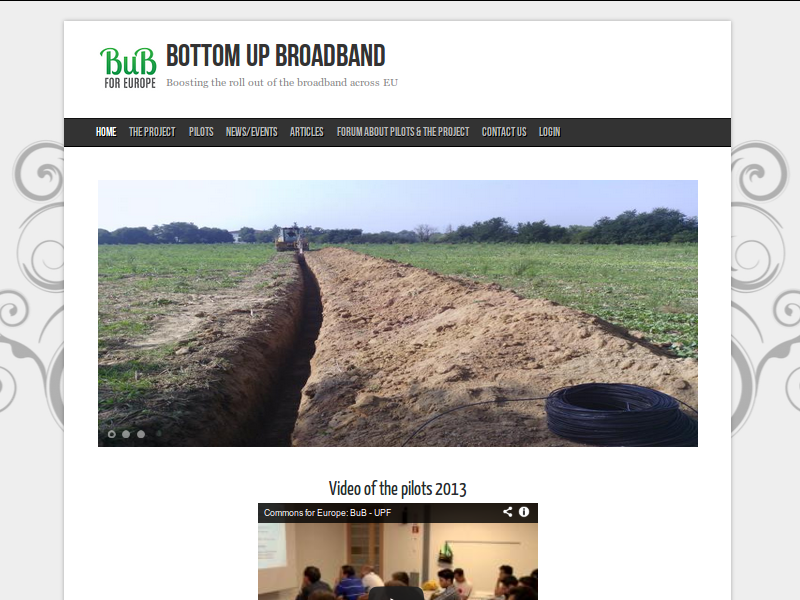
\includegraphics[width=0.95\linewidth]{sect2/figures/web_bub4EU_crop.png}
  \caption[BuBforEurope website]{Upper part of the BuBforEurope website main page.}
  \label{fig:bub_web}
\end{figure}

This website includes a section to manage the whole BuB pilots process. It includes a from to submit the pilot's proposals, another to submit fellows proposals, and a wiki for each proposal selected. Firgure~\ref{fig:bub_web} shows the pilots summary page.

\begin{figure}[H]
  \centering
  
\includegraphics[width=0.95\linewidth]{sect2/figures/web_bub4eu_pilots_crop.png}
  \caption[BuBforEurope website]{Upper part of the BuBforEurope website pilots section.}
  \label{fig:bub_web_pilots}
\end{figure}

This website has been mostly developed by Adriana Marti Hoppmann as part of her Final Degree Project. Her thesis\footnote{\url{http://upcommons.upc.edu/pfc/bitstream/2099.1/18721/1/89496.pdf}} includes a very accurate analysis of its design and implementation.


\subsubsection{tmpcommonsnet mailing list}

http://lists.sudoroom.org/listinfo/tmpcommonsnet

This mailing list, created in September 2013 at Sudoroom\footnote{A CN base in Oakland, USA, \url{https://sudoroom.org/}.} mailing list manager\footnote{\url{Mailman http://www.list.org/}.}, is meant for the BuB organisation that must be created as part of WP7 in the second reporting period. Its name has been chosen to reflect that the organisation project is a work in progress and that it has not even a name yet -idea stressed by the term \emph{tmp}.

Although it is been open since the beginning, its public announcement is foreseen by the beginning of next year, together with the organisation project announcement. At the moment it has around 25 subscribers of about 10 community networks.


\subsubsection{tmp-l2org wiki and pad}

http://dokuwiki.tmp-l2org.guifi.net/, http://etherpad.tmp-l2org.guifi.net/

These two tools, both hosted at a guifi.net server, complement the tmpcommonsnet mailing list. They have been set up in October 2013. While the pad\footnote{\url{https://github.com/ether/etherpad-lite}.} is conceived for taking notes (i.e. meeting notes) and for drafts, the wiki\footnote{\url{https://dokuwiki.org}.} is for meant for hosting more elaborate documentation.

Firgure~\ref{fig:l2org_wiki} shows the wiki main page.
 
\begin{figure}[H]
  \centering
  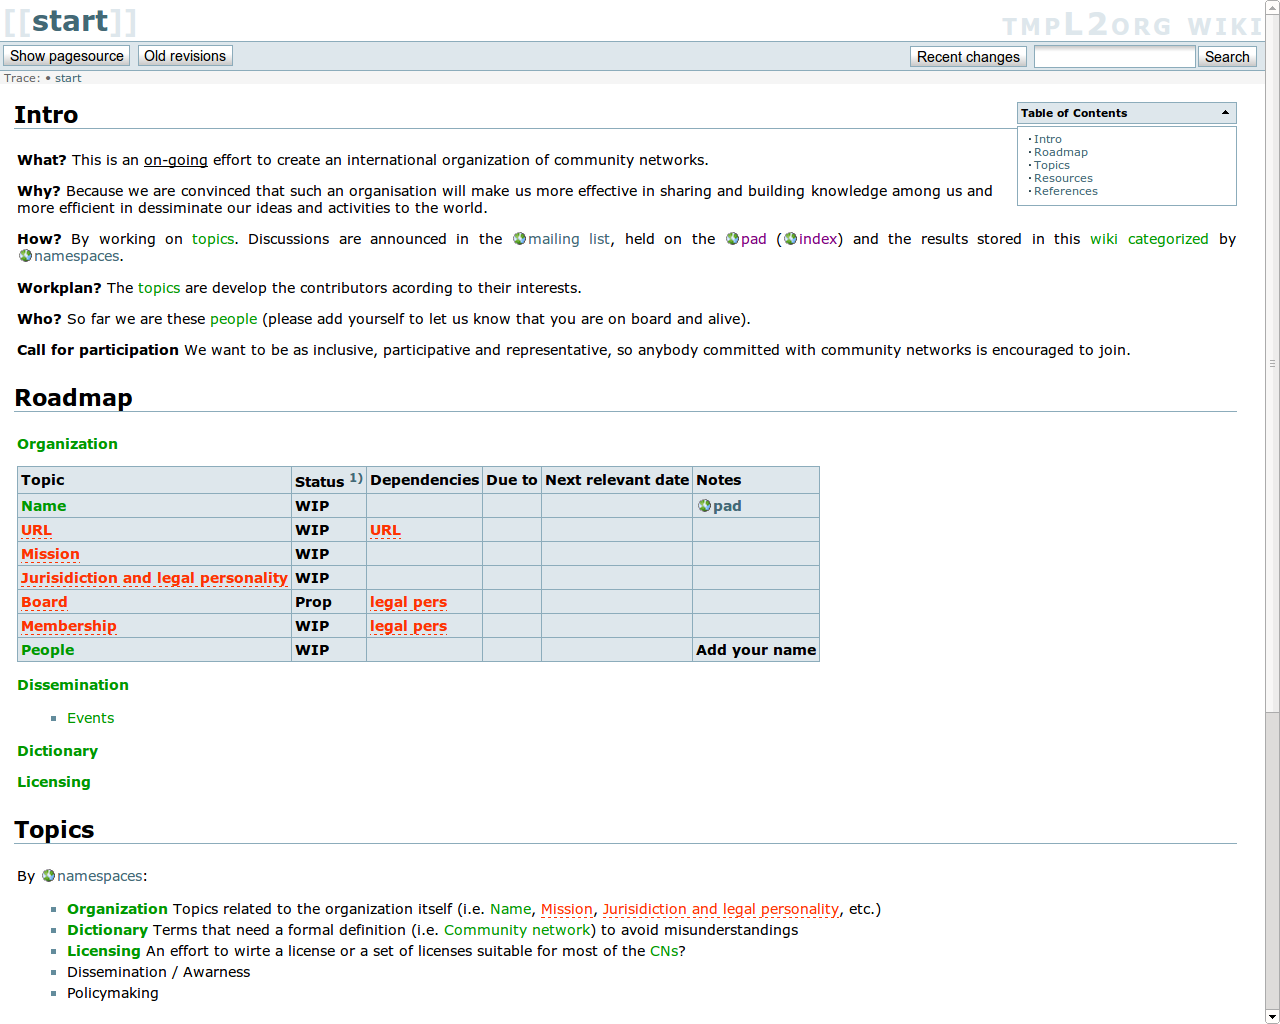
\includegraphics[width=0.95\linewidth]{sect2/figures/wiki_l2org.png}
  \caption[BuB organisation wiki]{Upper part of the BuB organisation wiki main page.}
  \label{fig:l2org_wiki}
\end{figure}


\subsection{Enlisting BuB organisations}

Three phases have been foreseen to create the organisation of BuB organisations (a so called second level organisation) and achieve the maximum enlistment and commitment:

\textbf{Initial}
This phase has the main following tasks.
\begin{itemize}
  \setlength{\itemindent}{2em}
  \item Identify BuB initiatives.
  \item Informal contacts and meetings with some of the BuB initiatives identified to introduce the idea and get feedback.
  \item Set up the collaboration tools needed.
  \item Characterisation of the organisation.
  \item Set the roadmap.
\end{itemize}


\textbf{Creation}
\begin{itemize}
  \setlength{\itemindent}{2em}
  \item Elaborate the issues identified during the initial phase.
  \item formalize the creation of the organisation.
  \item Announce the nascent organisation.
\end{itemize}


\textbf{Consolidation}
\begin{itemize}
  \setlength{\itemindent}{2em}
  \item Attend the new members requests.
  \item Amend detected problems.
  \item Do the mandated tasks.
\end{itemize}

During this year the initial phase has been started. As already planned, all the documentation is being gathered in the wiki. The following subsections present the results achieved.

%\hangindent=2em
%\hangafter=1
%\textbf{Identify BuB initiatives}
\subsubsection{Identify BuB initiatives}
Around 20 active BuB initiatives around the world have been identified\footnote{\url{http://dokuwiki.tmp-l2org.guifi.net/doku.php?id=organization:people}.}. This task is now frozen. During the Announcement of the organisation of the second phase further identification research will be done in order to reach as many initiatives as possible.


%\hangindent=2em
%\hangafter=1
%\textbf{Informal contacts and meetings with some of the BuB initiatives identified to introduce the idea and get feedback}
\subsubsection{Initial contacts and meetings}
We have already introduced the idea of a second level organisation to many BuB initiatives. All of them welcomed it and the following have started contributing:
\begin{itemize}
  \setlength{\itemindent}{2em}
  \item Free Network Foundation, USA
  \item Altermesh, Argentina
  \item Sudo Room, USA
  \item Wlan0, Solvenia.
  \item Ninux, Italy
  \item FreiFunk, Germany
\end{itemize}

The most relevant face-to-face meetings we have had are:
\begin{itemize}
  \setlength{\itemindent}{2em}
  \item \textbf{Barcelona, Catalonia, May 2013} Altermesh, Free Network Foundation, Pangea, guifi.net
  \item \textbf{Oakland, USA, September 2013} Sudo Room, Wlan0, Free Network Foundation, gufi.net
  \item \textbf{Berlin, October 2013} Altermesh, Free Network Foundation, Ninux, FreiFunk, guifi.net
\end{itemize}

Aside from CNs, we have had informal meetings with other players like Internet Exchange Points (NaMeX) and Regional Internet Registires (RIPE-NCC).

The most relevant events where we have presented our initiative are:
\begin{itemize}
  \setlength{\itemindent}{2em}
  \item Wireless Battle Mesh v5, Athens (Greece), March 2012
  \item International Summit for Wireless Community Networks 2012, Barcelona (Catalonia), October 2012
  \item Wireless Battle Mesh v6, Aalborg (Denmark), April 2013
  \item International Summit for Wireless Community Networks 2013, Berlin (Germany), October 2013
\end{itemize}


%\hangindent=2em
%\hangafter=1
%\textbf{Set up the collaboration tools required}
\subsubsection{Collaboration tools}
The tools already set up are described in Section~\ref{tools}. Together with some other tool hosted and maintained by a CN (like the VoIP service) are considered to be enough.

%\hangindent=2em
%\hangafter=1
%\textbf{Characterisation of the organisation}
\subsubsection{Characterisation of the organisation}
The following issues to be worked have been identified\footnote{\url{http://dokuwiki.tmp-l2org.guifi.net/doku.php#roadmap}.}.
\begin{itemize}
  \item Name
  \item URL
  \item Mission
  \item Membership
  \item jurisdiction and legal personality
  \item Board.
\end{itemize}
This is task where most of the efforts are currently focused.


% % %  \item Set the roadmap.
%
%
%meetings
%Attending events -> 
%
%
%
%FTTH council -> altre report
%
%
%
%\subsection{Events}
%
%Part of the research done has been on identifying the most important events related to BuB and attending them to learn from the others and to create awareness of our activity.
%
%The most relevant events attended since the beginning of the Common for Europe project are the following:
%
%\textbf{FTTH Conference 2013}
%\begin{description}
% \item[Organiser] FTTH Council Europe (http://www.ftthcouncil.eu/)
% \item[Description] 
%\end{description}
%
%\textbf{FTTH Conference 2013}
%\hangindent=2em
%\hangafter=1
%\textbf{Organiser}
%FTTH Council Europe (http://www.ftthcouncil.eu/)
%
%TODO TODO TODO TODO TODO TODO TODO TODO TODO TODO TODO TODO TODO TODO TODO TODO TODO TODO TODO TODO TODO TODO TODO TODO TODO TODO TODO TODO TODO TODO TODO TODO TODO TODO TODO TODO TODO TODO TODO TODO TODO TODO TODO TODO 
%
%TODO TODO TODO TODO TODO TODO TODO TODO TODO TODO TODO TODO TODO TODO TODO TODO TODO TODO TODO TODO TODO TODO TODO TODO TODO TODO TODO TODO TODO TODO TODO TODO TODO TODO TODO TODO TODO TODO TODO TODO TODO TODO TODO TODO 
%
%
%
%
%FTTH counsil
